\section{Реализация интеллектуальной системы мониторинга рисков и обеспечения безопасности путешественников}
\label{sec:development}

В данном разделе подробно описывается процесс программной реализации спроектированной системы, приводятся расширенные примеры исходного кода ключевых модулей на языках Python и Java, а также демонстрируются результаты работы пользовательского интерфейса. Разработка велась с применением современных практик непрерывной интеграции, контейнеризации и автоматизированного тестирования, что позволило обеспечить высокую надежность и расширяемость всех компонентов интеллектуальной платформы.

\subsection{Разработка модуля сбора и первичной обработки данных}

Модуль Fetcher является входной точкой системы и реализован на языке Python 3.12 с использованием асинхронной парадигмы программирования. Основная сложность реализации данного модуля заключалась в необходимости обработки огромных массивов данных проекта GDELT, которые публикуются в виде сжатых CSV-файлов каждые 15 минут и могут содержать информацию о тысячах событий одновременно.

Для обеспечения высокой производительности и минимизации задержек был разработан асинхронный клиент на базе библиотеки \textbf{httpx}, позволяющий параллельно загружать архивы событий и упоминаний. После загрузки данные передаются в конвейер обработки, реализованный с применением библиотеки \textbf{pandas}, которая обеспечивает векторизованную фильтрацию и очистку данных на низком уровне.

На рисунке~\ref{fig:code_gdelt_fetcher} представлен фрагмент кода асинхронного сервиса загрузки данных GDELT.

\trmcodefigure[34]{language=Python}{gdelt_fetcher.py}{асинхронного сервиса загрузки данных GDELT}{fig:code_gdelt_fetcher}

Ключевые особенности реализации модуля сбора данных:
\begin{itemize}
    \item применение асинхронных контекстных менеджеров для эффективного управления сетевыми соединениями и ресурсами операционной системы;
    \item использование векторизованных операций библиотеки \textbf{pandas} для быстрой фильтрации записей по пороговым значениям индекса Гольдштейна;
    \item реализация отказоустойчивой очереди сообщений на базе RabbitMQ, гарантирующей доставку идентификаторов событий в аналитический модуль;
    \item внедрение механизмов логирования и мониторинга состояния сетевых запросов для оперативного выявления сбоев на стороне источников данных;
    \item использование временных хранилищ для минимизации нагрузки на оперативную память при обработке файлов объемом в несколько сотен мегабайт.
\end{itemize}

Данный подход позволил сократить время от момента публикации данных в GDELT до начала их анализа нейронными сетями до 5--10 секунд, что является критически важным для систем экстренного оповещения.

\subsection{Реализация интеллектуального анализа событий}

Модуль интеллектуального анализа представляет собой высокотехнологичный конвейер на базе FastAPI, объединяющий классические методы обработки естественного языка и современные генеративные модели. Процесс анализа разделен на этапы извлечения контента, семантической классификации и реферирования, что позволяет гибко настраивать параметры каждой модели в зависимости от типа входных данных.

Для классификации угроз используется модель DeBERTa-v3-large, настроенная на задачу классификации без предварительного обучения на целевых классах. Это позволяет системе распознавать новые типы инцидентов (например, специфические киберугрозы или новые виды природных аномалий) без необходимости формирования обучающей выборки и дообучения весов нейронной сети.

Особое внимание уделено интеграции с локальной языковой моделью через программный интерфейс Ollama. Это обеспечивает полную автономность системы и исключает зависимость от внешних провайдеров, что критично для обеспечения конфиденциальности и снижения операционных затрат.

Для поддержки локализации в аналитический конвейер был добавлен этап определения языка исходного материала и генерации переводных версий ключевых полей события. На практике это означает, что после извлечения текста статьи модуль определяет язык источника, формирует базовую краткую сводку, а затем подготавливает локализованные варианты названия и описания для языков, поддерживаемых пользовательским интерфейсом. Такой подход позволяет не выполнять перевод во время каждого запроса к программному интерфейсу, а сохранять готовые версии в основной базе данных.

На рисунке~\ref{fig:code_intelligence_analyzer} представлен фрагмент кода модуля интеллектуального анализа событий с применением трансформеров и больших языковых моделей.

\trmcodefigure[38]{language=Python,basicstyle=\ttfamily\scriptsize}{intelligence_analyzer.py}{модуля интеллектуального анализа событий с применением трансформеров и больших языковых моделей}{fig:code_intelligence_analyzer}

Программные решения, внедренные в аналитический модуль:
\begin{itemize}
    \item использование библиотеки \textbf{transformers} для реализации высокоточной семантической классификации текстов на естественном языке;
    \item интеграция с локальным сервером Ollama через программный интерфейс в стиле REST для выполнения ресурсоемких задач реферирования на выделенных графических мощностях;
    \item ограничение входного контекста для большой языковой модели до 1000 символов с целью оптимизации времени инференса и предотвращения галлюцинаций модели;
    \item применение асинхронных вызовов к программным интерфейсам нейросетевых моделей для обеспечения параллельной обработки нескольких инцидентов одновременно;
    \item сохранение языка исходного материала и локализованных версий описания для дальнейшей выдачи пользователю без повторного инференса;
    \item реализация механизмов повторных попыток при взаимодействии с вычислительными модулями машинного обучения.
\end{itemize}

\subsection{Реализация серверной логики и геоинформационных компонентов}

Ядро системы, отвечающее за хранение данных, управление пользователями и выполнение пространственных запросов, реализовано на Java 21 с использованием фреймворка Spring Boot 3.3. Ключевым технологическим преимуществом является использование Hibernate Spatial, что позволяет оперировать геометрическими объектами непосредственно в коде приложения.

Для реализации логики геофенсинга~--- поиска пользователей, находящихся в зоне риска,~--- применяется специализированное расширение PostGIS. Это позволяет выполнять сложные математические вычисления на стороне СУБД, возвращая в приложение только готовый результат.

Сущность \textbf{EventEntity} описывает структуру инцидента в базе данных и одновременно обеспечивает поддержку локализованных полей и геопространственных типов. На рисунке~\ref{fig:code_event_entity} представлен фрагмент кода сущности \textbf{EventEntity}.

\trmcodefigure[36]{language=Java,basicstyle=\ttfamily\scriptsize}{event_entity.java}{сущности EventEntity}{fig:code_event_entity}

Поверх сущности построен слой репозиториев на базе JPA Criteria API. Метод \textbf{findEventsForMap} формирует пространственный запрос для выборки инцидентов в пределах видимой области карты с учетом порога опасности и активного языка интерфейса. На рисунке~\ref{fig:code_event_geofeature} представлен фрагмент кода репозитория пространственной выборки событий для карты.

\trmcodefigure[40]{language=Java,basicstyle=\ttfamily\scriptsize}{event_geofeature.java}{репозитория пространственной выборки событий для карты}{fig:code_event_geofeature}

Для отдачи геоданных клиентскому приложению реализован унифицированный контроллер \textbf{GeoServerController}, который агрегирует поставщиков геообъектов разных типов в один массовый эндпоинт. Такой подход позволяет фронтенду одним запросом получать сразу все слои карты. На рисунке~\ref{fig:code_geoserver_controller} представлен фрагмент кода контроллера \textbf{GeoServerController}.

\trmcodefigure[38]{language=Java,basicstyle=\ttfamily\scriptsize}{geoserver_controller.java}{контроллера GeoServerController}{fig:code_geoserver_controller}

Технические особенности реализации серверной части:
\begin{itemize}
    \item использование библиотеки JTS (Java Topology Suite) для выполнения точных геометрических вычислений на стороне приложения;
    \item применение аннотаций JPA и Hibernate Spatial для автоматического маппинга географических координат в типы данных PostGIS;
    \item реализация специализированных репозиториев на базе Criteria API для динамического построения пространственных запросов с фильтрами по пороговому уровню опасности, типу события и сроку актуальности;
    \item построение унифицированного программного интерфейса \textbf{/geoserver/batch}, агрегирующего разные слои геоданных через паттерн \textbf{GeofeatureProvider}, что упрощает добавление новых типов геообъектов в будущем;
    \item хранение локализованных заголовков и описаний событий в JSONB-полях PostgreSQL с выбором нужной версии непосредственно в SQL-запросе через \textbf{jsonb\_extract\_path\_text};
    \item внедрение механизмов кэширования результатов гео-запросов для снижения нагрузки на дисковую подсистему базы данных при частом обновлении координат.
\end{itemize}

\subsection{Реализация системы почтовых уведомлений}

Для гарантированной доставки информации об угрозах в системе реализована рассылка по электронной почте, рассматриваемая как резервный и юридически значимый канал коммуникации. Сервис уведомлений на Java использует \textbf{Spring Mail} для взаимодействия с почтовым сервером и формирования HTML-шаблонов писем.

На рисунке~\ref{fig:code_email_notification} представлен фрагмент кода сервиса отправки почтовых оповещений.

\trmcodefigure[28]{language=Java}{email_notification.java}{сервиса отправки почтовых оповещений}{fig:code_email_notification}

Отдельным этапом разработки стала верстка шаблонов уведомлений, которые должны быть читаемы на любых устройствах и почтовых клиентах. Исходные HTML-шаблоны хранятся в каталоге \textbf{html-snippets} проекта~--- по одному файлу на каждую поддерживаемую локаль. На рисунке~\ref{fig:email_notification} представлено содержимое почтовых уведомлений о риске безопасности на английском и русском языках. Обе языковые версии размещены на одном экране и используют единую табличную верстку с инлайн-стилями, что обеспечивает совместимость с большинством современных почтовых клиентов, включая Microsoft Outlook, Gmail и Apple Mail. В верхней части письма расположен фирменный градиентный заголовок с уровнем угрозы, ниже~--- блок ключевых параметров события (регион, время, расстояние от пользователя), за ним следуют аналитическая сводка, нумерованный список рекомендуемых действий и кнопка перехода в систему мониторинга.

\begin{figure}[!ht]
    \centering
    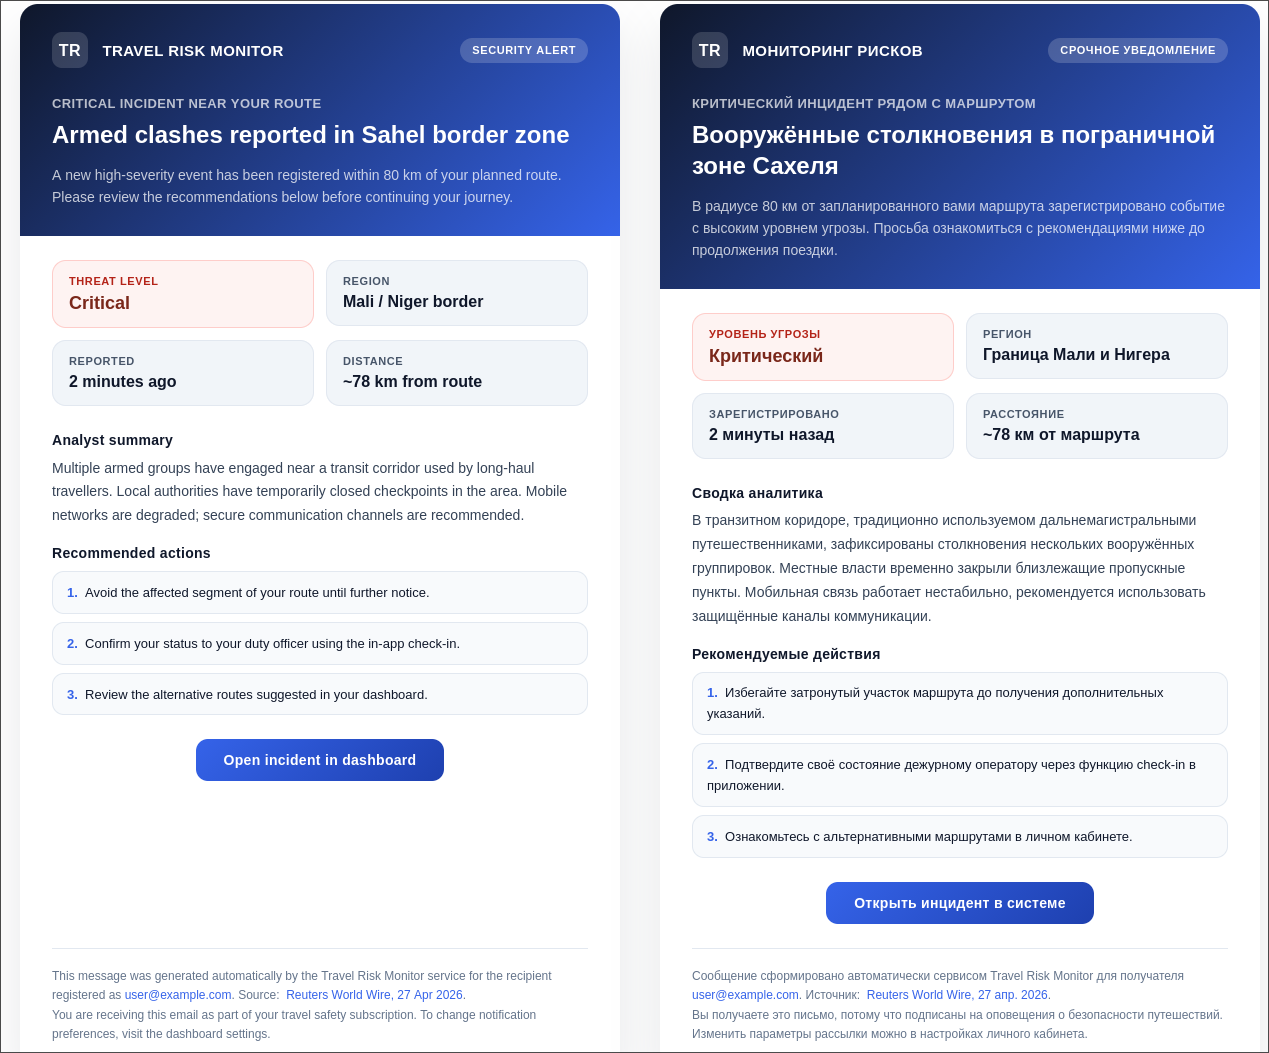
\includegraphics[width=\linewidth]{picture/email_notification.png}
    \caption{Содержимое почтовых уведомлений о риске безопасности на английском и русском языках}
    \label{fig:email_notification}
\end{figure}

\subsection{Разработка клиентского интерфейса и ГИС-компонентов}

Фронтенд-приложение построено на базе React 19 и Redux Toolkit. Для отрисовки карты в React-компонентах используется библиотека \textbf{react-map-gl}, которая инкапсулирует вызовы движка MapLibre GL JS и позволяет декларативно подключать слои данных. Выбор библиотеки обусловлен открытой лицензией, отсутствием платных ограничений и поддержкой векторных тайлов.

Локализация клиентского интерфейса реализована через словари переводов на базе \textbf{i18next} и передачу выбранной локали в запросах к серверной части. При открытии карты или страницы события клиентская часть получает уже подготовленные локализованные поля, поэтому пользователю не требуется ждать выполнения машинного перевода на клиенте, а все формулировки остаются согласованными между веб-интерфейсом и почтовыми уведомлениями.

Обращение к серверу геоданных оформлено в виде единого запроса в массовый эндпоинт \textbf{/api/v1/geoserver/batch}, что позволяет за один сетевой обмен получать все слои карты, видимые в текущей области. На рисунке~\ref{fig:code_fetch_map_batch} представлен фрагмент кода клиентского запроса к массовому эндпоинту геоданных.

\trmcodefigure[28]{language=JavaScriptES}{fetch_map_batch.js}{клиентского запроса к массовому эндпоинту геоданных}{fig:code_fetch_map_batch}

Главный компонент карты декларативно объявляет слои инцидентов, маршрутов путешественника и пользовательских остановок. При перемещении области просмотра автоматически перезапрашиваются геоданные, а при клике по точке открывается всплывающее окно и боковая панель с подробностями события. На рисунке~\ref{fig:code_map_view} представлен фрагмент кода главного компонента карты.

\trmcodefigure[42]{language=JavaScriptES,basicstyle=\ttfamily\scriptsize}{map_view.js}{главного компонента карты}{fig:code_map_view}

Аналитическая логика модуля прокладки маршрутов реализована на стороне клиента и опирается на формулу гаверсинусов, обеспечивающую корректный расчет дистанции между географическими координатами на сфере. Дополнительно поддерживается расчет расстояния от точки события до ближайшего сегмента маршрута, что используется для определения зоны риска вокруг проложенного пути. На рисунке~\ref{fig:code_haversine} представлен фрагмент кода расчета расстояния по формуле гаверсинусов и до сегмента маршрута.

\trmcodefigure[34]{language=JavaScriptES}{haversine.js}{расчета расстояния по формуле гаверсинусов и до сегмента маршрута}{fig:code_haversine}

Перед началом работы с системой пользователь проходит процедуру аутентификации. Окно входа выполнено в едином стиле приложения и поддерживает мгновенное переключение языка интерфейса и темы оформления. После успешной авторизации пользователь попадает на главный экран, представляющий собой интерактивную карту мира с активными инцидентами. Цвет и размер маркеров рассчитываются на основе уровня опасности, а вокруг каждой точки отрисовывается мягкий ореол, имитирующий пульсирующее поведение и упрощающий визуальное восприятие плотности рисков. На рисунке~\ref{fig:login_screen} представлено окно входа в систему, а на рисунке~\ref{fig:main_map_view}~--- главное окно системы с визуализацией карты инцидентов.

\begin{figure}[!ht]
    \centering
    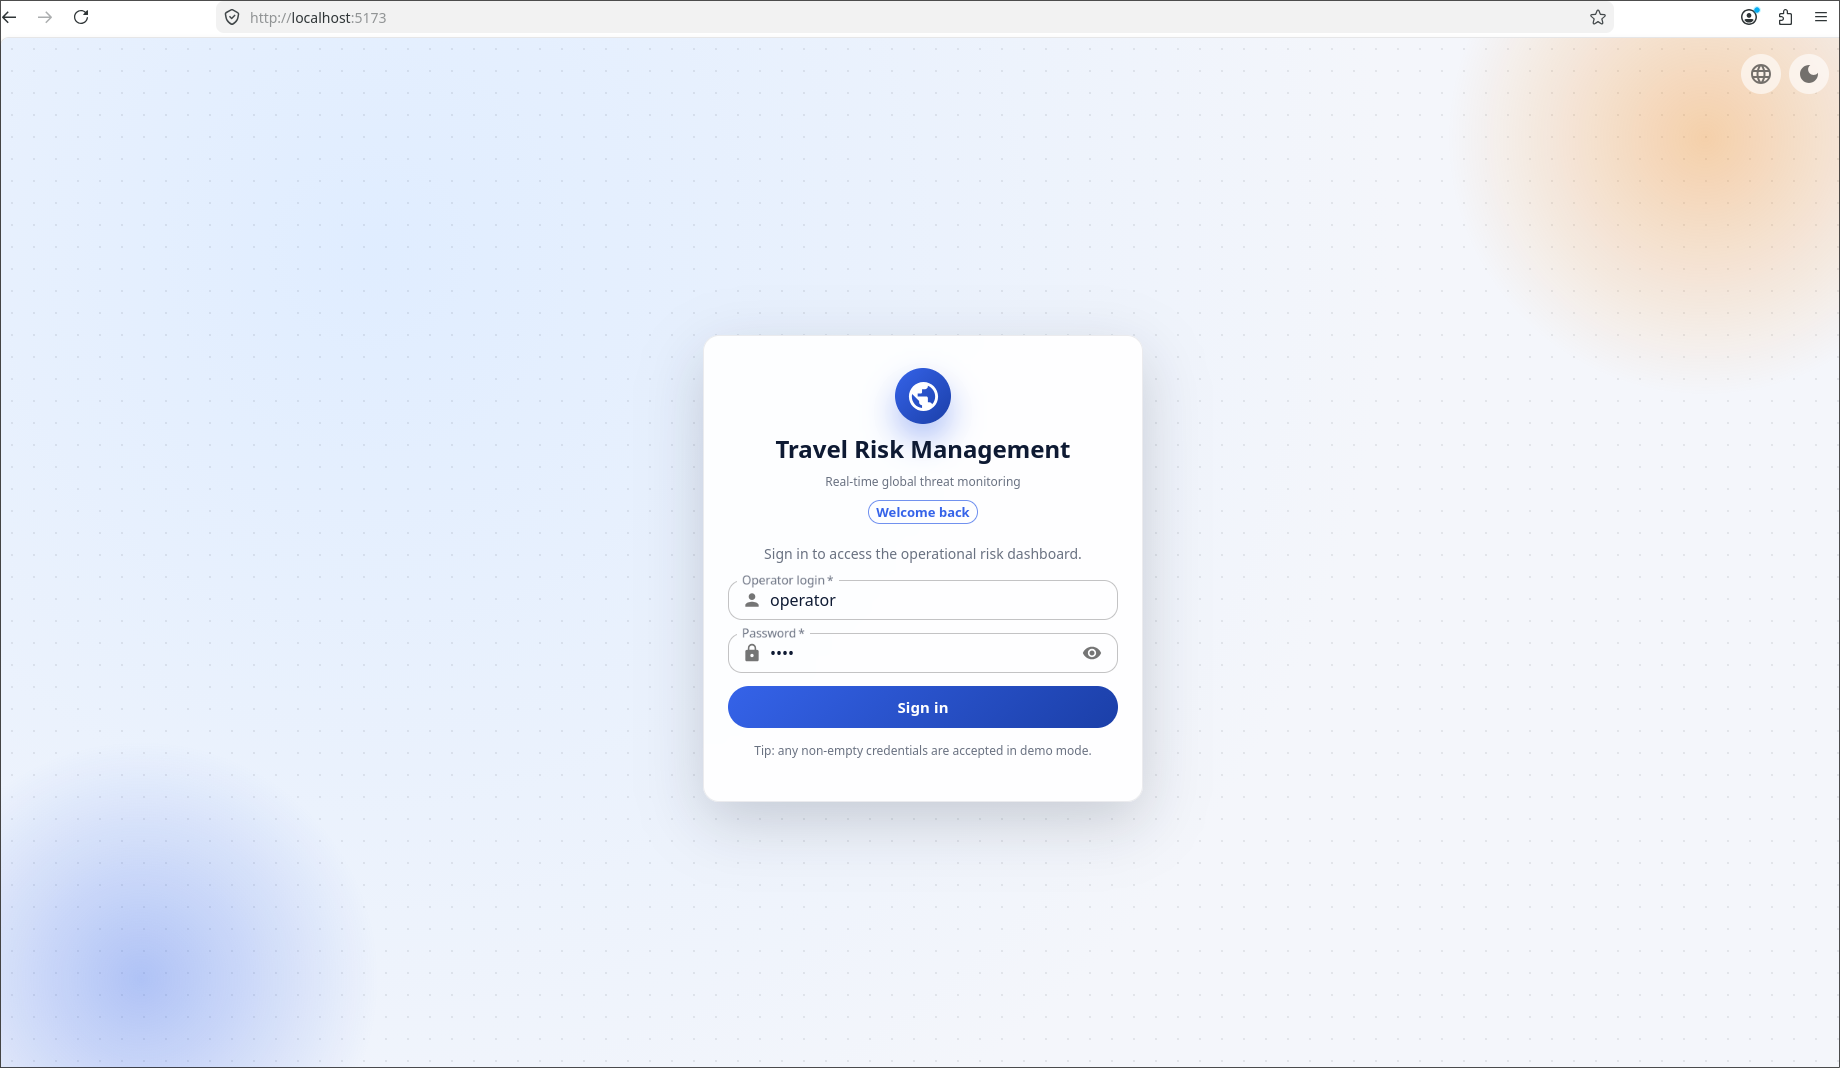
\includegraphics[width=1\textwidth]{picture/login_screen.png}
    \caption{Окно входа в систему}
    \label{fig:login_screen}
\end{figure}

\begin{figure}[!ht]
    \centering
    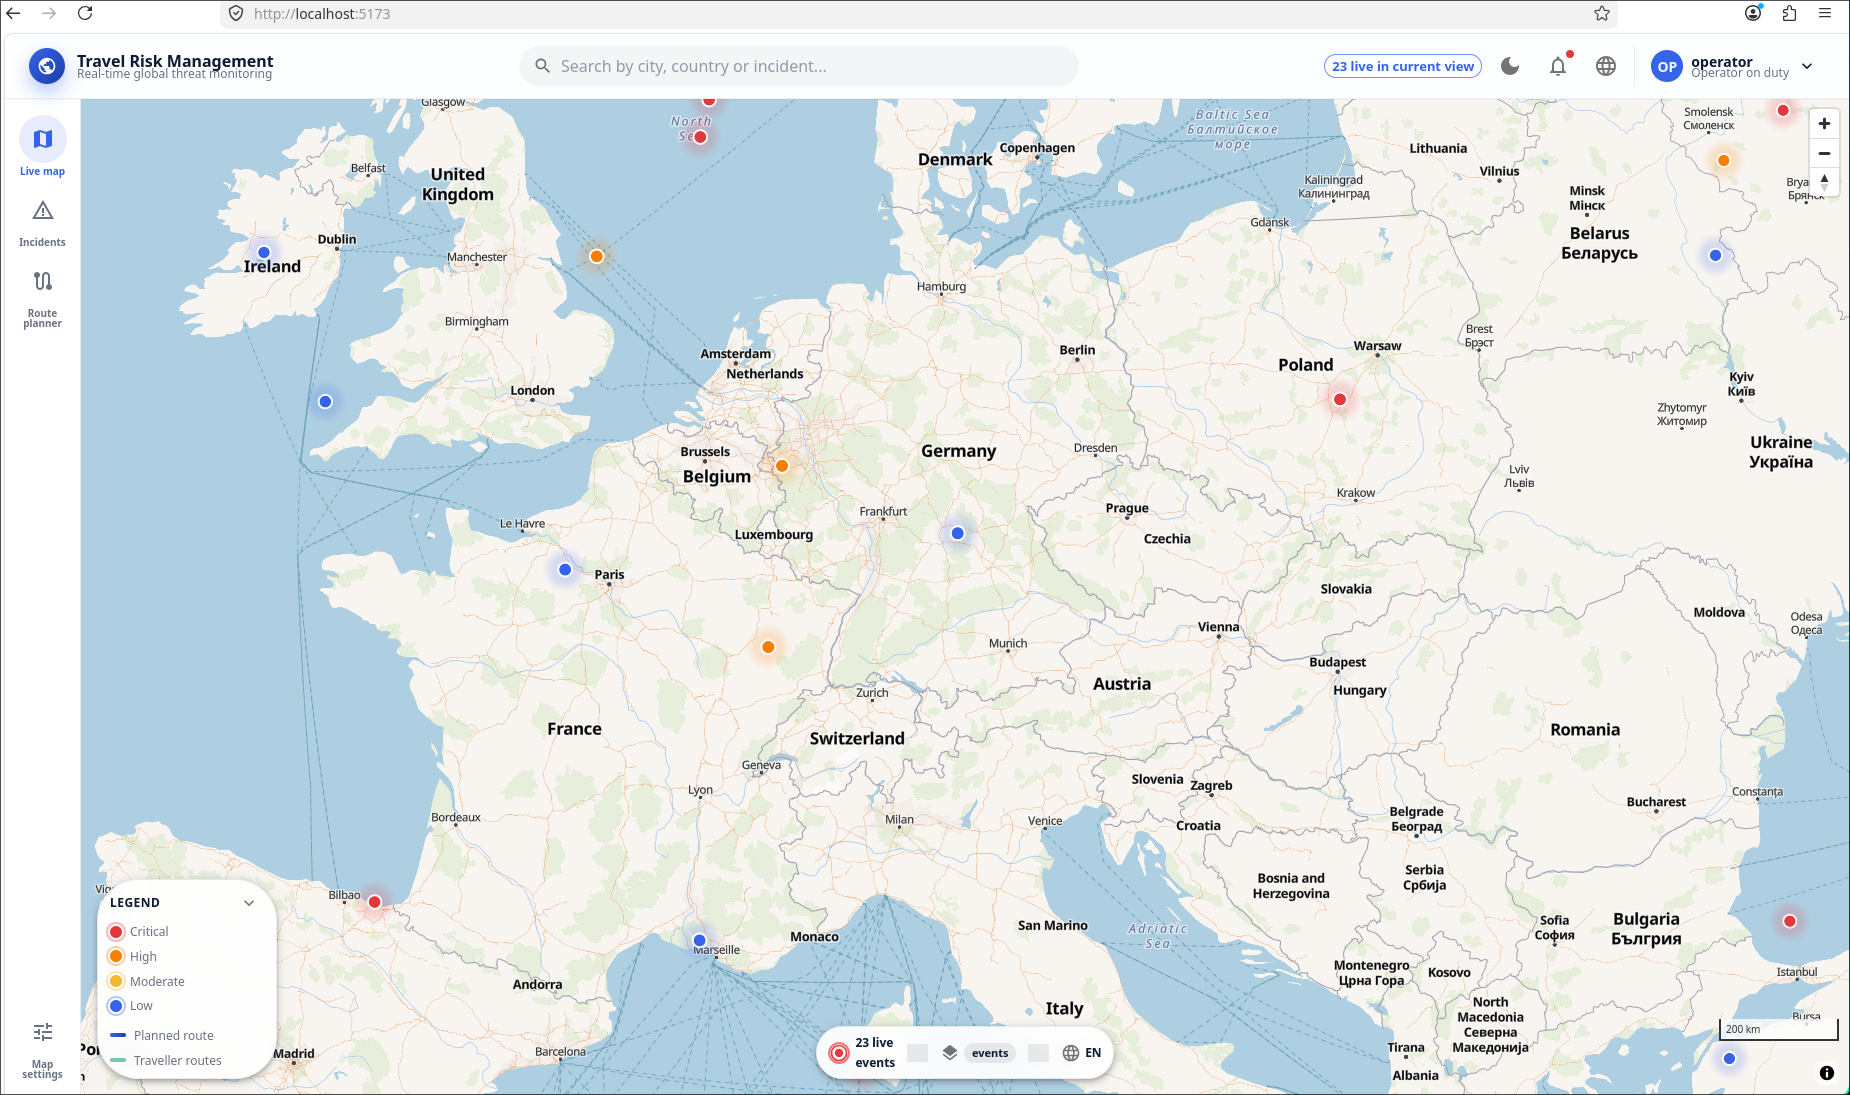
\includegraphics[width=1\textwidth]{picture/main_map_interface.png}
    \caption{Главное окно системы с визуализацией карты инцидентов}
    \label{fig:main_map_view}
\end{figure}

Для детального изучения отдельного инцидента в интерфейсе реализована страница события с локализованным заголовком, описанием, уровнем угрозы, временем публикации и ссылкой на исходный материал. На странице приводятся также агрегированный уровень риска, регион и тип инцидента, аналитическая сводка и блок с рекомендуемыми действиями для оператора. Поскольку текстовое содержимое формируется на этапе аналитической обработки и сохраняется сразу для всех поддерживаемых локалей, переключение языка происходит мгновенно и не требует выполнения машинного перевода в момент открытия карточки. На рисунке~\ref{fig:event_page} представлена страница события с локализованным содержимым.

\begin{figure}[!ht]
    \centering
    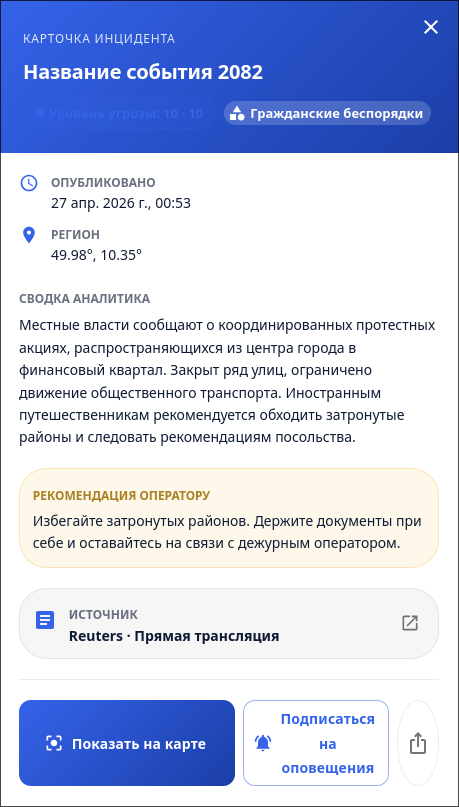
\includegraphics[width=0.85\linewidth]{picture/event_page_ru.png}
    \caption{Страница события с локализованным содержимым}
    \label{fig:event_page}
\end{figure}

\subsection{Разработка интерфейса прокладки и анализа маршрута}

Помимо мониторинга текущих инцидентов система предоставляет инструмент планирования маршрута, в котором пользователь последовательно проходит четыре шага мастера: добавление точек, настройка расписания, анализ безопасности и сохранение маршрута. Дополнительно поддерживается вкладка с ранее сохраненными маршрутами, что позволяет вернуться к редактированию или дублированию существующего пути. Анимированные переходы между шагами и интерактивная установка точек прямо на карте делают работу с модулем интуитивной даже для пользователей без специальной подготовки.

На рисунке~\ref{fig:route_step1} представлен первый шаг мастера прокладки маршрута~--- добавление путевых точек. Для каждой точки отображается порядковый номер, локализованное название, координаты и быстрые действия, позволяющие центрировать карту на точке либо удалить ее. Дополнительно поддерживается режим, в котором новая точка автоматически создается по клику на карте, что особенно удобно при первичной прокладке маршрута в незнакомом регионе. На втором шаге пользователь указывает даты пребывания в каждой точке, итоговую длительность поездки и расчетную дистанцию; эти данные сохраняются в локальное состояние клиента до явного подтверждения сохранения маршрута.

\begin{figure}[!ht]
    \centering
    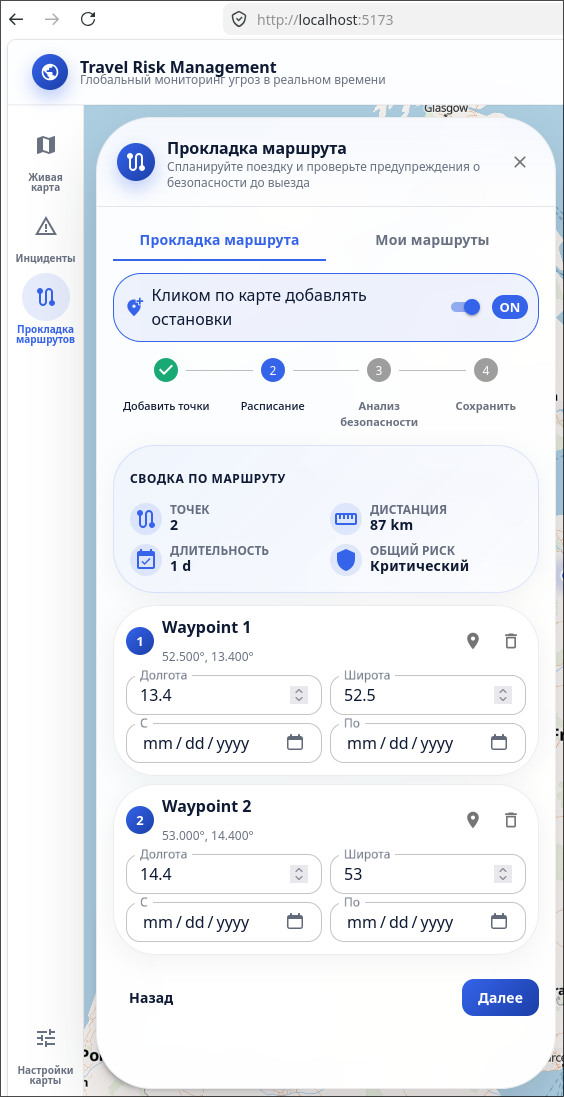
\includegraphics[width=0.92\linewidth]{picture/route_planning_step1_waypoints.png}
    \caption{Первый шаг мастера прокладки маршрута~--- добавление путевых точек}
    \label{fig:route_step1}
\end{figure}

На рисунке~\ref{fig:route_step3} представлен третий шаг мастера прокладки маршрута~--- анализ пересечений с активными инцидентами. На стороне клиента вычисляется минимальное расстояние от каждого активного инцидента до сегментов маршрута, после чего инциденты, попавшие в настраиваемый радиус буфера, выводятся в виде списка предупреждений. Для удобства восприятия каждое предупреждение сопровождается цветным индикатором уровня опасности и расстоянием от линии маршрута. Радиус буфера задается пользователем при помощи бегунка и может варьироваться от 10 до 500 километров, что позволяет адаптировать строгость проверки под требования конкретной поездки.

\begin{figure}[!ht]
    \centering
    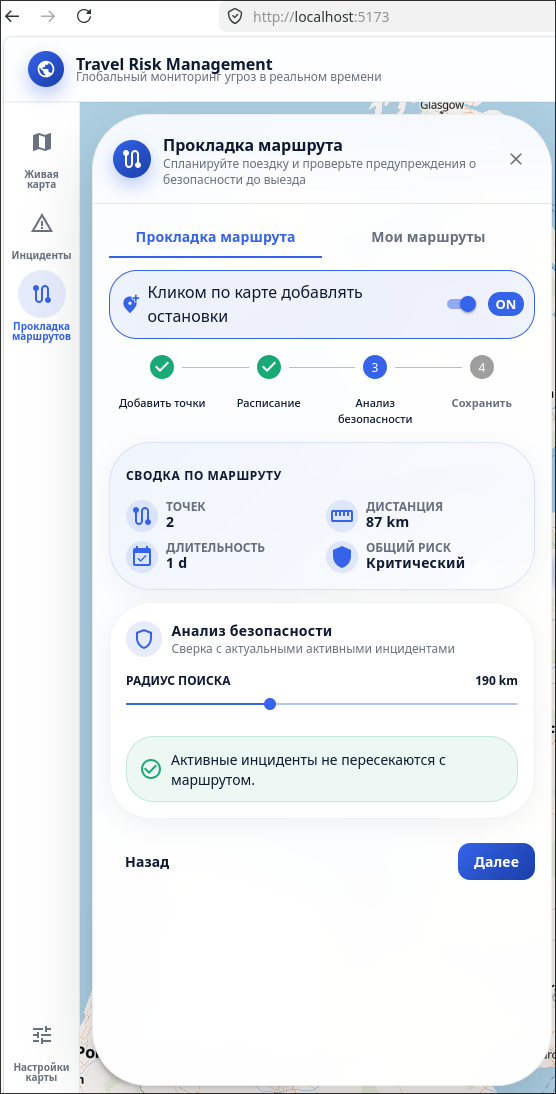
\includegraphics[width=0.92\linewidth]{picture/route_planning_step3_safety.png}
    \caption{Третий шаг мастера прокладки маршрута~--- анализ пересечений с активными инцидентами}
    \label{fig:route_step3}
\end{figure}

Логика анализа маршрута сосредоточена в компоненте \textbf{RouteRiskPanel}: список кандидатов формируется из данных о текущих видимых инцидентах и резервных шаблонных событиях, после чего фильтруется по расстоянию от линии маршрута и сортируется по близости к ней. На рисунке~\ref{fig:code_route_risk} представлен фрагмент кода компонента \textbf{RouteRiskPanel}, реализующего фильтрацию инцидентов по расстоянию до маршрута.

\trmcodefigure[32]{language=JavaScriptES}{route_risk.js}{компонента RouteRiskPanel, реализующего фильтрацию инцидентов по расстоянию до маршрута}{fig:code_route_risk}

После прохождения анализа безопасности пользователь переходит на финальный шаг мастера~--- сохранение маршрута с вводом названия, итоговой сводкой и подтверждающим уведомлением системы. В случае недоступности серверного эндпоинта клиентское приложение помечает маршрут как сохраненный локально и отображает соответствующую информационную пометку, что обеспечивает непрерывность пользовательского сценария даже при кратковременных сбоях сети.

Все ранее сохраненные пути доступны на отдельной вкладке. Каждая карточка маршрута содержит название, количество точек, расчетную дистанцию, агрегированный уровень риска и быстрые действия~--- показать на карте либо продублировать для редактирования. При отсутствии у пользователя сохраненных маршрутов или при недоступности соответствующего эндпоинта система демонстрирует тематическую заглушку с примерами популярных маршрутов, что облегчает первичное знакомство с возможностями модуля. На рисунке~\ref{fig:route_my_routes} представлен список ранее сохраненных пользователем маршрутов.

\begin{figure}[!ht]
    \centering
    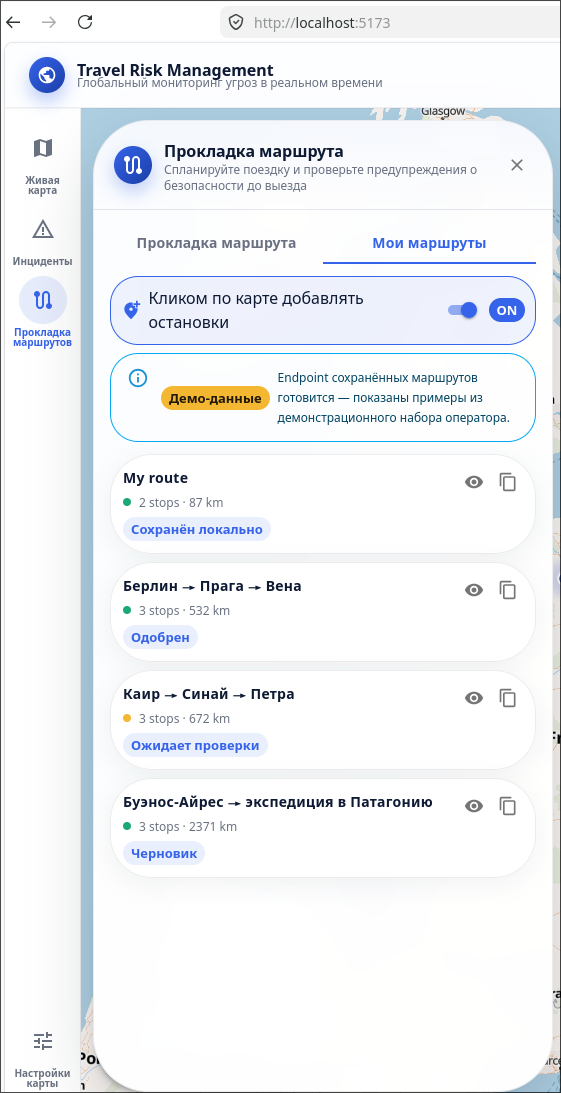
\includegraphics[width=0.75\textwidth]{picture/route_planning_my_routes.png}
    \caption{Список ранее сохраненных пользователем маршрутов}
    \label{fig:route_my_routes}
\end{figure}

\subsection{Вывод по реализации}

В результате дипломного проектирования был разработан и успешно протестирован полноценный программный комплекс интеллектуального мониторинга рисков, который полностью отвечает всем функциональным требованиям. В ходе реализации были решены сложные инженерные задачи, связанные с обработкой больших данных и интеграцией нейросетевых моделей в реальный бизнес-процесс.

Основные результаты этапа разработки:
\begin{itemize}
    \item реализован высокопроизводительный асинхронный модуль сбора данных на Python, способный обрабатывать поток новостей из проекта GDELT в реальном времени;
    \item разработан интеллектуальный аналитический конвейер, использующий модели DeBERTa-v3 для классификации и большую языковую модель Qwen 2.5 для автоматического реферирования инцидентов;
    \item создана надежная серверная часть на Java со встроенной поддержкой геопространственных данных и механизмов асинхронного геофенсинга;
    \item внедрена база данных PostgreSQL с расширением PostGIS, обеспечивающая высокую скорость выполнения пространственных запросов на пересечение маршрутов;
    \item разработан современный клиентский интерфейс на базе WebGL, обеспечивающий плавную визуализацию глобальной карты рисков, локализованное отображение карточек событий и интерактивную прокладку маршрута с анализом безопасности на стороне клиента;
    \item реализована система почтовых рассылок, гарантирующая доставку локализованной информации о безопасности конечному пользователю.
\end{itemize}

Все компоненты системы интегрированы в рамках единой событийно-ориентированной микросервисной архитектуры, что обеспечивает высокий потенциал для дальнейшего горизонтального масштабирования и внедрения новых прогностических модулей.
